\documentclass{report}

\usepackage[a4paper, total={6in, 8in}, margin=1in,footskip=0.25in]{geometry}
\usepackage{amsmath, amsthm, amssymb, booktabs, chemfig, gensymb, graphicx, float, pgfplots, upgreek, siunitx, multirow, multicol, setspace, longtable}
\renewcommand{\familydefault}{\sfdefault}
\usepackage[hidelinks]{hyperref}
\newcommand{\perthousand}{‰}
\newcommand{\micro}{µ}
\renewcommand{\printatom}[1]{\ensuremath{\mathrm{#1}}}
\usepackage[chemgreek=mhchem]{chemmacros}
\chemsetup[phases]{pos=sub}
\chemsetup[reactants]{concentration-unit=\moLar}
\chemsetup{
  formula = mhchem, % or mhchem
}

\DeclareSIUnit{\solub}{\unit[per-mode=symbol]{\gram\per\qty{100}{\gram}\,\ce{H2O}}}

\setlength{\parindent}{0pt}
\setlength{\parskip}{0.8em}

\pgfplotsset{compat=1.18}

\graphicspath{{../../Images/}}

\title{\Huge Year 12 Chemistry \\
	\begin{Large}
		Module 7 Depth Study
	\end{Large}}
\author{L. Cheung}

\tolerance=1
\emergencystretch=\maxdimen
\hyphenpenalty=10000
\hbadness=10000

\begin{document}
	\setstretch{1.25}

	\DeclareSIUnit{\molar}{\mole\per\liter}
	\DeclareSIUnit{\enthalpy}{\kJ\per\mole}
	\maketitle
	\newpage

\section*{Chapter 8 Review}

	\begin{enumerate}
		\item \textbf{Explain why carbon is the basis for so many compounds.}
			\subitem Carbon readily bonds to other carbon atoms, and has 4 valence electrons. This allows it to bond with many other elements and is therefore used as a base for compounds.

		\item \textbf{Draw electron dot diagrams to show how single, double and triple carbon-carbon bonds form.}
			\begin{center}
				\charge{0=\:, 90=\., 180=\., 270=\.}{C} \charge{0=\., 90=\., 270=\.}{C} \\
				\charge{0=\:\:,180=\:}{C} \charge{0=\:}{C} \\
				\charge{180=\., 0=\:\:\:}{C} \charge{0=\.}{C}
			\end{center}
		    
		\item \textbf{Draw diagrams and name the geometrical shapes formed when carbon atoms have:}
		\begin{enumerate}
			\item \textit{four single bonds}
				\begin{center}
					\chemfig{C(-[2])(-[6])(-[8])-[4]}
				\end{center}

				Forms a tetrahedron

			\item \textit{one double and two single bonds}
				\begin{center}
					\chemfig{C(=[0])(-[3])(-[5])}
				\end{center}

				Forms a trigonal planar

			\item \textit{two double bonds}
				\begin{center}
					\chemfig{C(=[4])(=[0])}
				\end{center}

				Forms a linear structure

			\item \textit{one triple and one single bond.}
				\begin{center}
					\chemfig{C(-[4])(~[0])}
				\end{center}

				Forms a linear structure

		\end{enumerate}
		    
		\item \textbf{Describe, with examples, the difference between saturated and unsaturated compounds.}

			Compounds are considered saturated when all carbon atoms have single bonds. For example, methane only has single bonds, hence is saturated. An unsaturated compound has at least one double or triple bonded carbon atom. An example of such is carbon dioxide.
		    
		\item \textbf{Describe, with examples, the difference between aromatic and aliphatic compounds.}

			Aliphatic compounds have open chained structures, ie. the carbon chain has a ends, for example butane. These can also be branched compounds, with alkyls attached to the main branch.

			Aromatic have one or more benzene rings, with the benzene compound being the most basic
		    
\newpage

		\item \textbf{For each of the families of hydrocarbons (alkanes, alkenes and alkynes):}

			\begin{itemize}
				\item \textit{give the general formula}
				\item \textit{write the molecular and structural formula for the first five in the series; for the alkenes and alkynes, have the double and triple bond on the first carbon.}
			\end{itemize}
				
			\begin{table}[H]
				\centering
				\setstretch{1.25}
				\begin{tabular}{p{3cm}|p{3cm}|p{10cm}}
					\textbf{Alkanes} (\ce{C_{n}H_{2n+2}})	& \textbf{Molecular Formula}	& \textbf{Structural Formula}			\\ \hline
										&				&						\\
										& \ce{CH4}			& \chemfig{C(-[2]H)(-[4]H)(-[6]H)(-[8]H)}	\\
										&				&						\\
										& \ce{C2H6}			& \chemfig{C(-[2]H)(-[4]H)(-[6]H) - C(-[2]H)(-[0]H)(-[6]H)}
										&				&						\\
										& \ce{C3H8}			& \chemfig{C(-[2]H)(-[4]H)(-[6]H)-C(-[2]H)(-[6]H)-C(-[2]H)(-[6]H)(-[0]H)}	\\
										&				&						\\
										& \ce{C4H10}			& \chemfig{C(-[2]H)(-[4]H)(-[6]H)-C(-[2]H)(-[6]H)-C(-[2]H)(-[6]H)-C(-[2]H)(-[6]H)(-[0]H)}	\\
										&				&						\\
										& \ce{C5H12}			& \chemfig{C(-[2]H)(-[4]H)(-[6]H)-C(-[2]H)(-[6]H)-C(-[2]H)(-[6]H)-C(-[2]H)(-[6]H)-C(-[2]H)(-[6]H)(-[0]H)}	\\
				\end{tabular}
			\end{table}

			\begin{table}[H]
				\centering
				\setstretch{1.25}
				\begin{tabular}{p{3cm}|p{3cm}|p{10cm}}
					\textbf{Alkenes} (\ce{C_{n}H_{2n}})	& \textbf{Molecular Formula}	& \textbf{Structural Formula}			\\ \hline
										&				&						\\
										& \ce{C2H4}			& \chemfig{C(-[3]H)(-[5]H) = C(-[1]H)(-[7]H)}	\\
										&				&						\\
										& \ce{C3H6}			& \chemfig{C(-[3]H)(-[5]H) = C(-[2]H) - C(-[2]H)(-[6]H)(-[0]H)} \\
										&				&						\\
										& \ce{C4H8}			& \chemfig{C(-[3]H)(-[5]H) = C(-[2]H) - C(-[2]H)(-[6]H) - C(-[2]H)(-[6]H)(-[8]H)} \\
										&				&						\\
										& \ce{C5H10}			& \chemfig{C(-[3]H)(-[5]H) = C(-[2]H) - C(-[2]H)(-[6]H) - C(-[2]H)(-[6]H) - C(-[2]H)(-[6]H)(-[0]H)} \\
										&				&						\\
										& \ce{C6H12}			& \chemfig{C(-[3]H)(-[5]H) = C(-[2]H) - C(-[2]H)(-[6]H) - C(-[2]H)(-[6]H) - C(-[2]H)(-[6]H) - C(-[2]H)(-[6]H)(-[8]H)} \\
				\end{tabular}
			\end{table}

			\begin{table}[H]
				\centering
				\setstretch{1.25}
				\begin{tabular}{p{3cm}|p{3cm}|p{10cm}}
					\textbf{Alkynes} (\ce{C_{n}H_{2n-2}})	& \textbf{Molecular Formula}	& \textbf{Structural Formula}			\\ \hline
										&				&						\\
										& \ce{C2H2}			& \chemfig{C(-[4]H) ~ C(-[0]H)}			\\
										&				&						\\
										& \ce{C3H4}			& \chemfig{C(-[4]H) ~ C - C(-[2]H)(-[6]H)(-[0]H)} \\
										&				&						\\
										& \ce{C4H6}			& \chemfig{C(-[4]H) ~ C - C(-[2]H)(-[6]H) - C(-[2]H)(-[6]H)(-[0]H)} \\
										&				&						\\
										& \ce{C5H8}			& \chemfig{C(-[4]H) ~ C - C(-[2]H)(-[6]H) - C(-[2]H)(-[6]H) - C(-[2]H)(-[6]H)(-[8]H)} \\
										&				&						\\
										& \ce{C6H10}			& \chemfig{C(-[4]H) ~ C - C(-[2]H)(-[6]H) - C(-[2]H)(-[6]H) - C(-[2]H)(-[6]H) - C(-[2]H)(-[6]H)(-[8]H)} \\
				\end{tabular}
			\end{table}
		    
		\item \textbf{Name the following hydrocarbons.}
			\begin{enumerate}
				\item 2-methylbutane
				\item 4-ethyl-2,3,3-trimethylpropane
				\item pent-2-ene
				\item 2,4,4-trimethylpent-2-ene
				\item 3,5-dimethylhex-1-yne
				\item 4-methylhept-2-yne
				\item 1,2-dichloro-3,3-difluoropentane
				\item 1,1,4-trichloro-1,2,4-trifluorohept-2-ene
			\end{enumerate}

		\newpage

		\item \textbf{Draw structural formula for the following molecules.}
			\begin{enumerate}
				\item 1,1-dichloroethane
					\subitem \chemfig{C(-[2]Cl)(-[4]H)(-[6]Cl) - C(-[2]H)(-[6]H)(-[0]H)} \\

				\item 2,3-dimethylhexane
					\subitem \chemfig{C(-[2,0.6]H)(-[4,0.6]H)(-[6,0.6]H) - C(-[2]C(-[0,0.6]H)(-[2,0.6]H)(-[4,0.6]H))(-[6,0.6]H) - C(-[6]C(-[0,0.6]H)(-[6,0.6]H)(-[4,0.6]H))(-[2,0.6]H) - C(-[2,0.6]H)(-[6,0.6]H) - C(-[2,0.6]H)(-[6,0.6]H) - C(-[2,0.6]H)(-[6,0.6]H)(-[0,0.6]H)} \\

				\item 2,2,6-trimethyl-3-octene
					\subitem \chemfig{C(-[2,0.6]H)(-[4,0.6]H)(-[6,0.6]H) - C(-[2] C(-[0,0.6]H)(-[2,0.6]H)(-[4,0.6]H))(-[6] C(-[0,0.6]H)(-[6,0.6]H)(-[4,0.6]H)) - C(-[2,0.6]H) = C(-[2,0.6]H) - C(-[2,0.6]H)(-[6,0.6]H) - C(-[2]C(-[0,0.6]H)(-[2,0.6]H)(-[4,0.6]H))(-[6,0.6]H) - C(-[2,0.6]H)(-[6,0.6]H) - C(-[0,0.6]H)(-[2,0.6]H)(-[6,0.6]H)} \\

				\item 2,3-dimethyl-3-ethyl-1-pentene
					\subitem \chemfig{C(-[3,0.6]H)(-[5,0.6]H) = C(-[2]C(-[0,0.6]H)(-[2,0.6]H)(-[4,0.6]H)) - C(-[2]C(-[0,0.6]H)(-[2,0.6]H)(-[4,0.6]H))(-[6]C(-[4,0.6]H)(-[0,0.6]H)(-[6]C(-[4,0.6]H)(-[6,0.6]H)(-[0,0.6]H))) - C(-[2,0.6]H)(-[6,0.6]H) - C(-[2,0.6]H)(-[6,0.6]H)(-[0,0.6]H)} \\

				\item 4,5-dimethyl-2-hexyne
					\subitem \chemfig{C(-[2,0.6]H)(-[4,0.6]H)(-[6,0.6]H) - C ~ C - C(-[2]C(-[2,0.6]H)(-[4,0.6]H)(-[0,0.6]H))(-[6,0.6]H) - C(-[6]C(-[0,0.6]H)(-[4,0.6]H)(-[6,0.6]H))(-[2,0.6]H) - C(-[0,0.6]H)(-[2,0.6]H)(-[6,0.6]H)} \\

				\newpage

				\item 3-ethyl-3-methyl-1-pentyne
					\subitem \chemfig{C(-[4,0.6]H) ~ C - C(-[2]C(-[2]C(-[0,0.6]H)(-[2,0.6]H)(-[4,0.6]H))(-[0,0.6]H)(-[4,0.6]H))(-[6]C(-[0,0.6]H)(-[4,0.6]H)(-[6,0.6]H)) - C(-[2,0.6]H)(-[6,0.6]H) - C(-[2,0.6]H)(-[6,0.6]H)(-[0,0.6]H)} \\

				\item 2,3,4-trichloro-2,3-difluoroheptane
					\subitem \chemfig{C(-[2,0.6]H)(-[4,0.6]H)(-[6,0.6]H) - C(-[2,0.6]{Cl})(-[6,0.6]{F}) - C(-[2,0.6]{Cl})(-[6,0.6]{F}) - C(-[2,0.6]{Cl})(-[6,0.6]H) - C(-[2,0.6]H)(-[6,0.6]H) - C(-[2,0.6]H)(-[6,0.6]H) - C(-[2,0.6]H)(-[0,0.6]H)(-[6,0.6]H)} \\

				\item 1,1,1-tribromo-2,2,2-trifluoroethane
					\subitem \chemfig{C(-[2]Br)(-[4]Br)(-[6]Br) - C(-[2]F)(-[0]F)(-[6]F)} \\
			\end{enumerate}

		\item \textbf{Draw the following molecules, identify why they are named incorrectly and give the correct name.}
			\begin{enumerate}
				\item 5-hexene
					\subitem \chemfig{CH_3 - CH_2 - CH_2 - CH_2 - CH = CH_2}\\

					The number to indicate the location of the double bond should be the smallest value possible. Correction: hex-1-ene

				\item 2,2-dimethyl-4-heptene
					\subitem \chemfig{CH_3 - C(-[2]CH_3)(-[6]CH_3) - CH_2 - CH = CH_2 - CH_2 - CH_3} \\

					The number to indicate the location of the double bond should be the smallest value possible. Correction: 6,6-dimethylhept-3-ene

				\item 1,1-dichloro-2-bromo-3-butene
					\subitem \chemfig{CH(-[3]Cl)(-[5]Cl) - CH(-[2]Br) - CH = CH_2} \\

					The number to indicate the location of the double bond should be the smallest value possible. "Bromo" component should come before "chloro" to maintain alphabetical order. Correction: 3-bromo-4,4-dichlorobut-1-ene
			\end{enumerate}

		\item \textbf{Explain whether the following pairs of structures represent isomers.}
			\begin{enumerate}
				\item No - they are the same compound of 2-methylbutane.
				\item Yes - they are positional isomers 3-methylpentane and 2-methylpentane
				\item No - they are the same molecule 3-methylpentane
				\item Yes - they are positional isomers 2,3-dimethylpentane and 2,4-dimethylpentane
			\end{enumerate}

		\item \textbf{Draw and name all possible isomers of:}
			\begin{enumerate}
				\item pentane
					\begin{table}[H]
						\centering
						\setstretch{1.25}
						\begin{tabular}{p{4cm}|p{8cm}}
							Name			& Diagram		\\ \hline
							pentane			& \chemfig{CH_3 - CH_2 - CH_2 - CH_2 - CH_3}	\\
							\\
							2-methylbutane		& \chemfig{CH_3 - CH(-[6]CH_3) - CH_2 - CH_3}	\\
							\\
							2,2-dimethylpropane	& \chemfig{CH_3 - C(-[2]CH_3)(-[6]CH_3) - CH_3}	\\ \end{tabular}
					\end{table}

				\item the alkene \ce{C6H12} with the double bond staying between the first and second carbon atoms
					\begin{table}[H]
						\centering
						\setstretch{1.25}
						\begin{tabular}{p{4cm}|p{8cm}}
							Name			& Diagram			\\ \hline
							\\
							hex-1-ene		& \chemfig{CH_2 = CH - CH_2 - CH_2 - CH_2 - CH_3}	\\
							\\
							2-methylpent-1-ene	& \chemfig{CH_2 = C(-[6]CH_3) - CH_2 - CH_2 - CH_3}	\\
							\\
							3-methylpent-1-ene	& \chemfig{CH_2 = CH - CH(-[6]CH_3) - CH_2 - CH_3}	\\
							\\
							2,3-dimethylbut-1-ene	& \chemfig{CH_2 = C(-[2]CH_3) - CH(-[2]CH_3) - CH_3}	\\
							\\
							3,3-dimethylbut-1-ene	& \chemfig{CH_2 = CH - C(-[2]CH_3)(-[6]CH_3) - CH_3}	\\
						\end{tabular}
					\end{table}

				\item the alkene \ce{C6H12} with the double bond staying between the second and third carbon atoms
					\begin{table}[H]
						\centering
						\setstretch{1.25}
						\begin{tabular}{p{4cm}|p{8cm}}
							Name			& Diagram			\\ \hline
							\\
							hex-2-ene		& \chemfig{CH_3 - CH = CH - CH_2 - CH_2 - CH_3}	\\
							\\
							2-methylpent-2-ene	& \chemfig{CH_3 - C(-[6]CH_3) = CH - CH_2 - CH_3}	\\
							\\
							3-methylpent-2-ene	& \chemfig{CH_3 - CH = CH(-[6]CH_3) - CH_2 - CH_3}	\\
							\\
							2,3-dimethylbut-2-ene	& \chemfig{CH_3 - C(-[2]CH_3) = C(-[2]CH_3) - CH_3}	\\
						\end{tabular}
					\end{table}

				\item \textbf{the alkyne \ce{C5H8} with the triple bond staying between the first and second carbon atoms.}
					\begin{table}[H]
						\centering
						\setstretch{1.25}
						\begin{tabular}{p{4cm}|p{8cm}}
							Name			& Diagram			\\ \hline
							\\
							pent-1-yne		& \chemfig{CH ~ C - CH_2 - CH_2 - CH_3}		\\
							\\
							3-methylbut-1-yne	& \chemfig{CH ~ C - CH(-[2]CH_3) - CH_3}	\\
						\end{tabular}
					\end{table}
			\end{enumerate}

		\item \textbf{Using specific organic molecules, distinguish between chain and position isomers.}
			\subitem Positional isomers are molecules that share the same carbon skeleton with alkyl groups rearranged. For example the following compounds 2-methylpentane and 3-methylpentane share the same five long carbon skeleton, however have methyl groups on different carbon atoms.
				\begin{center}
					\chemfig{CH_3 - CH(-[2]CH_3) - CH_2 - CH_2 - CH_3}
					
					\chemfig{CH_3 - CH_2 - CH(-[2]CH_3) - CH_2 - CH_3}
				\end{center}

			\subitem Chain isomers involve rearrangement of the central carbon chain. For example, pentane and 2-methylbutane both have the chemical formula \ce{C5H12} however pentane has a longer carbon chain of five compared to the 2-methylbutane
				\begin{center}
					\chemfig{CH_3 - CH_2 - CH_2 - CH_2 - CH_3}

					\chemfig{CH_3 - CH(-[2]CH_3) - CH_2 - CH_3}
				\end{center}

\newpage

		\item \textbf{Pentane and 2,2-dimethylpropane are isomers.}
			\begin{enumerate}
				\item \textit{Identify the type of isomer that is formed here.}

					\subitem Chain isomer

				\item \textit{Draw both molecules}

					Pentane

					\begin{center}
						\chemfig{CH_3 - CH_2 - CH_2 - CH_2 - CH_3}
					\end{center}

					2,2-dimethylpropane

					\begin{center}
						\chemfig{CH_3 - C(-[2]CH_3)(-[6]CH_3) - CH_3}
					\end{center}

				\item \textit{Predict and explain which isomer will have a higher boiling point.}
					
					\subitem Pentane has a longer carbon chain that allows more dispersion forces to occur in comparison to 2,2-dimethylpropane. Hence it will most likely have a higher boiling point.
			\end{enumerate}
		
		\item \textbf{The table below shows the boiling points for some alkenes.}

			\begin{enumerate}
				\item \textit{Calculate the molecular weight for each alkene and place into the table.}

					\begin{table}[H]
						\centering
						\setstretch{1.25}
						\begin{tabular}{p{3cm}|p{4.5cm}|p{4.5cm}}
							\textbf{Alkene}		& \textbf{Molecular Weight}	& \textbf{Boiling Point ($\degree C$)}	\\ \hline
							Ethene			& 28.05				& -104					\\
							Propene			& 42.08				& -48					\\
							but-1-ene		& 56.10				& -6					\\
							pent-1-ene		& 70.13				& 30					\\
							hex-1-ene		& 84.16				& 64					\\
							hept-1-ene		& 98.18				& 94					\\
							oct-1-ene		& 112.2				& 121					\\
						\end{tabular}
					\end{table}

				\item \textit{Graph the molecular weight against the boiling point.}

					\begin{figure}[H]
						\centering
						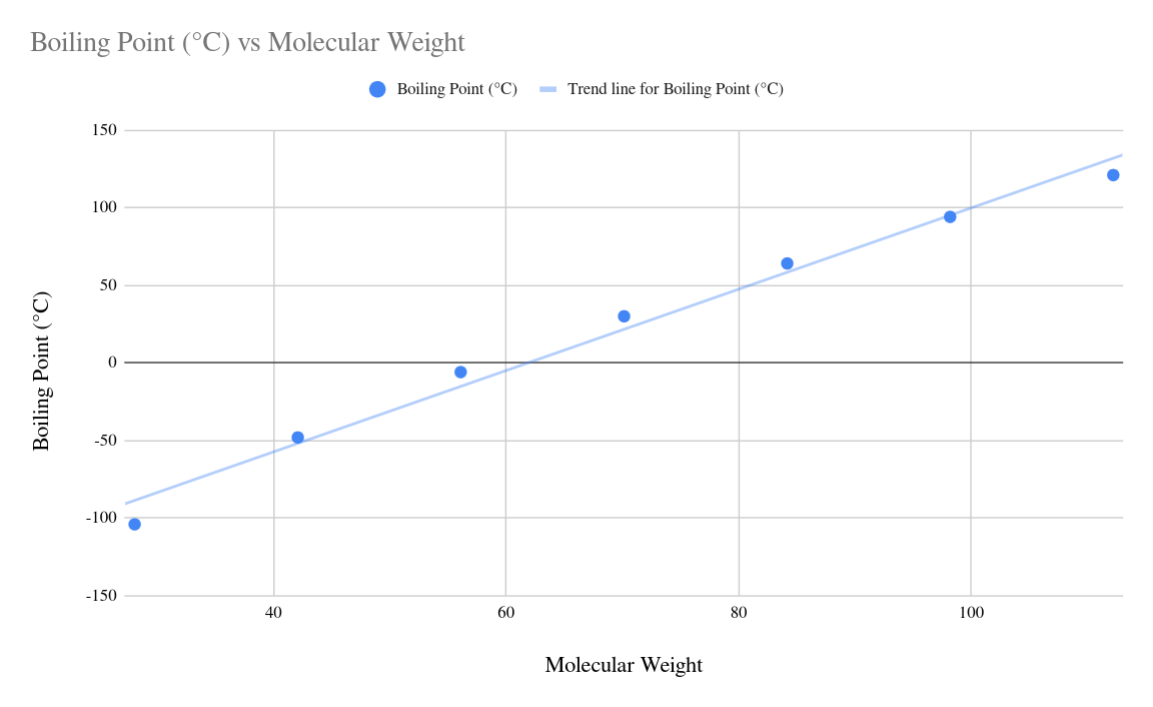
\includegraphics[width=15cm]{boiling_point_over_molecular_mass.png}
					\end{figure}

				\item \textit{Describe the trend shown on the graph.}

					There is a linear relationship between boiling point and molecular weight.

				\item \textit{Explain the trend in terms of intermolecular bonding.}

					Molecules with higher molecular masses have more atoms and can therefore induce more dispersion forces. More energy is required to break these bonds, hence molecules with higher molecular masses have higher boiling points than those of lower molecular mass.
			\end{enumerate}

		\item \textbf{Compound X has a boiling point of −6°C. Compound Y has a boiling point of 12°C. Compound Z has a boiling point of −55°C. All compounds are from the same homologous series.}

			\begin{enumerate}
				\item \textit{List the compounds in order of increasing molecular weight.}

					Compound Z, compound X, compound Y

				\item \textit{Explain your answer to part (a)}

					All 3 compounds are in the same homologous series and therefore share similar chemical formulae. Therefore, compounds with higher molecular weight will have higher boiling points
			\end{enumerate}

		\item \textbf{A compound has a relatively low boiling point, but is able to conduct electricity and is soluble in water. Is it likely to be a hydrocarbon? Justify your answer.}

			No. Hydrocarbons are non-polar and have no dipole charge and therefore cannot conduct electricity.

	\end{enumerate}

\newpage

\section*{Chapter 9 Review}

	\begin{enumerate}
		\item \textbf{Identify the functional group in each of the following compounds.}
			
			\begin{enumerate}
				\item Hydroxyl
				\item Carboxyl
				\item Amine
				\item Ester
				\item Carbonyl
				\item Carbonyl
				\item Amide
			\end{enumerate}

		\item \textbf{In general, in organic formulae an R group is often used. Explain what the R group represents.}

			The R group represents a general molecule.

		\item \textbf{Identify the functional group, draw its structure and give the general formula for alcohols, aldehydes, ketones and carboxylic acids.}
			
			\begin{table}[H]
				\centering
				\setstretch{1.25}
				\begin{tabular}{p{3cm}|p{3cm}|p{5cm}|p{3cm}}
					\textbf{Group}			& \textbf{Functional Group}		& \textbf{Structure}			& \textbf{General Formula}	\\ \hline
					Alcohol				& Hydroxyl				& \chemfig{-OH}				& \ce{C_{n}H_{2n+1}OH}		\\
									&					&					&				\\
					Aldehyde			& Carbonyl				& \chemfig{-C(=[2]O) - H}		& \ce{C_{n}H_{2n}O}		\\
									&					&					&				\\
					Ketone				& Carbonyl				& \chemfig{-C(-[2]O) -} 		& \ce{C_{n}H_{2n}O}		\\
									&					&					&				\\
					Carboxylic Acid			& Carbonyl				& \chemfig{-C(=[2]O) - OH} 		& \ce{C_{n}H_{2n}O2}		\\
				\end{tabular}
			\end{table}

		\item \textbf{Distinguish between an amine and amide in terms of structure and physical properties.}

			Amines are a functional group with a nitrogen atom and a lone pair in the form \ce{-NH2}. Amides form when the \ce{-OH} part of carboxylic acids is replaced by an amine functional group. Due to their \ce{N-H} bonds, both amines and amides have strong hydrogen bonding intermolecular forces. However, amides have a more polar functional group and therefore have higher boiling and melting points in comparison to that of amines.

		\item \textbf{For each of the following molecules, identify the homologous series it belongs to and write its correct IUPAC name.}
			\begin{enumerate}
				\item Alcohol, butan-2-ol
				\item Amide, N-methylethanamide
				\item Carboxylic acid, propanoic acid
				\item Amide, propanamide
				\item Ketone, 5-ethylhept-3-one
				\item Alcohol, 3-methylpentan-3-ol
			\end{enumerate}

		\item \textbf{Draw structural formulae for the following:}
			\begin{enumerate}
				\item 2-heptanol
					\subitem \chemfig{CH_3 - CH_2(-[2]OH) - CH_2 - CH_2 - CH_2 - CH_2 - CH_3} \\

				\item 4,5-dimethyl-2-hexanone
					\subitem \chemfig{CH_3 - C(=[2]O) - CH_2 - CH_2(-[2]CH_3) - CH_2(-[2]CH_3) - CH_3} \\

				\item 2-ethylbutanoic acid
					\subitem \chemfig{CH_3 - CH_2 - CH_2(-[2]CH_2(-[2]CH_3)) - C(=[1]O)(-[-1]OH)} \\

				\item 3-ethyl-1-hexanol
					\subitem \chemfig{CH_2(-[2]OH) - CH_2 - CH_2(-[6]CH_2(-[6]CH_3)) - CH_2 - CH_2 - CH_3} \\

				\item pentanamide
					\subitem \chemfig{C(-[4]NH_2)(=[2]O) - CH_2 - CH_2 - CH_2 - CH_3} \\

				\item 3-heptanamine
					\subitem \chemfig{CH_3 - CH_2 - CH(-[2]NH2) - CH_2 - CH_2 - CH_2 - CH_3} \\

				\item N-methylpropanamide
					\subitem \chemfig{C(-[4]N(-[-3]H)(-[3]CH_3))(=[2]O) - CH_2 - CH_2 - CH_3} \\

				\item 2-fluorobutanal
					\subitem \chemfig{CH(=[2]O) - CH(-[2]F) - CH_2 - CH_3} \\

				\item 3-methyl-2-butanone
					\subitem \chemfig{CH_3 - CH(=[2]O) - CH(-[2]CH_3) - CH_3} \\
			\end{enumerate}

		\item \textbf{Identify one alcohol, one aldehyde, and one carboxylic acid that have common names. Draw each molecule and give its correct IUPAC name.}
			
			Isopropyl alcohol (2-propanol)

				\begin{center}
					\chemfig{CH_3 - CH(-[2]OH) - CH_3}
				\end{center}

			Methanal (formaldehyde)

				\begin{center}
					\chemfig[angle increment = 30]{C(=[3]O)(-[-1]H)(-[-5]H)}
				\end{center}

			Acetic acid (ethanoic acid)

				\begin{center}
					\chemfig{CH_3 - C(=[1]O)(-[-1]H)}
				\end{center}

		\item \textbf{Draw structural formulae for the following and give the systematic names for:}
			\begin{enumerate}
				\item \textit{all isomers with molecular formula \ce{C3H8O}}
					
					\begin{table}[H]
						\centering
						\setstretch{1.25}
						\begin{tabular}{p{3cm}|p{9cm}}
							\textbf{Systematic Name}	& \textbf{Structural Formula}		\\ \hline
											&					\\
							Propan-1-ol			& \chemfig{CH_2(-[2]OH) - CH_2 - CH_3}	\\
											&					\\
							Propan-2-ol			& \chemfig{CH_3 - CH(-[2]OH) - CH_3}	\\
						\end{tabular}
					\end{table}

				\item \textit{carboxylic acids with molecular formula \ce{C4H8O}}

					\begin{table}[H]
						\centering
						\setstretch{1.25}
						\begin{tabular}{p{3cm}|p{9cm}}
							\textbf{Systematic Name}	& \textbf{Structural Formula}		\\ \hline
											&					\\
							Butanoic acid			& \chemfig{CH_3 - CH_2 - CH_2 - C(-[1]OH)(=[-1]O)}	\\
											&					\\
							2-methylpropanoic acid		& \chemfig{CH_3 - CH(-[-2]CH_3) - C(-[1]OH)(=[-1]O)}	\\
						\end{tabular}
					\end{table}

				\item \textbf{Compare the intermolecular forces and relative boiling points of the following classes of organic compounds.}

					\begin{enumerate}
						\item \textit Alkanes and alcohols
						\item \textit Carboxylic acids and aldehydes
						\item \textit Alcohols and aldehydes
						\item \textit Amines and amides
					\end{enumerate}

			\end{enumerate}
	\end{enumerate}
\end{document}

